\section{Referencia del Archivo /media/docs/progra/c++/compiladores1/proy2/godzilla/src/colaerr.c}
\label{colaerr_8c}\index{/media/docs/progra/c++/compiladores1/proy2/godzilla/src/colaerr.c@{/media/docs/progra/c++/compiladores1/proy2/godzilla/src/colaerr.c}}
Implementacion de la cola almacenadora de errores . 

{\tt \#include \char`\"{}colaerr.h\char`\"{}}\par


Dependencia gr\'{a}fica adjunta para colaerr.c:\begin{figure}[H]
\begin{center}
\leavevmode
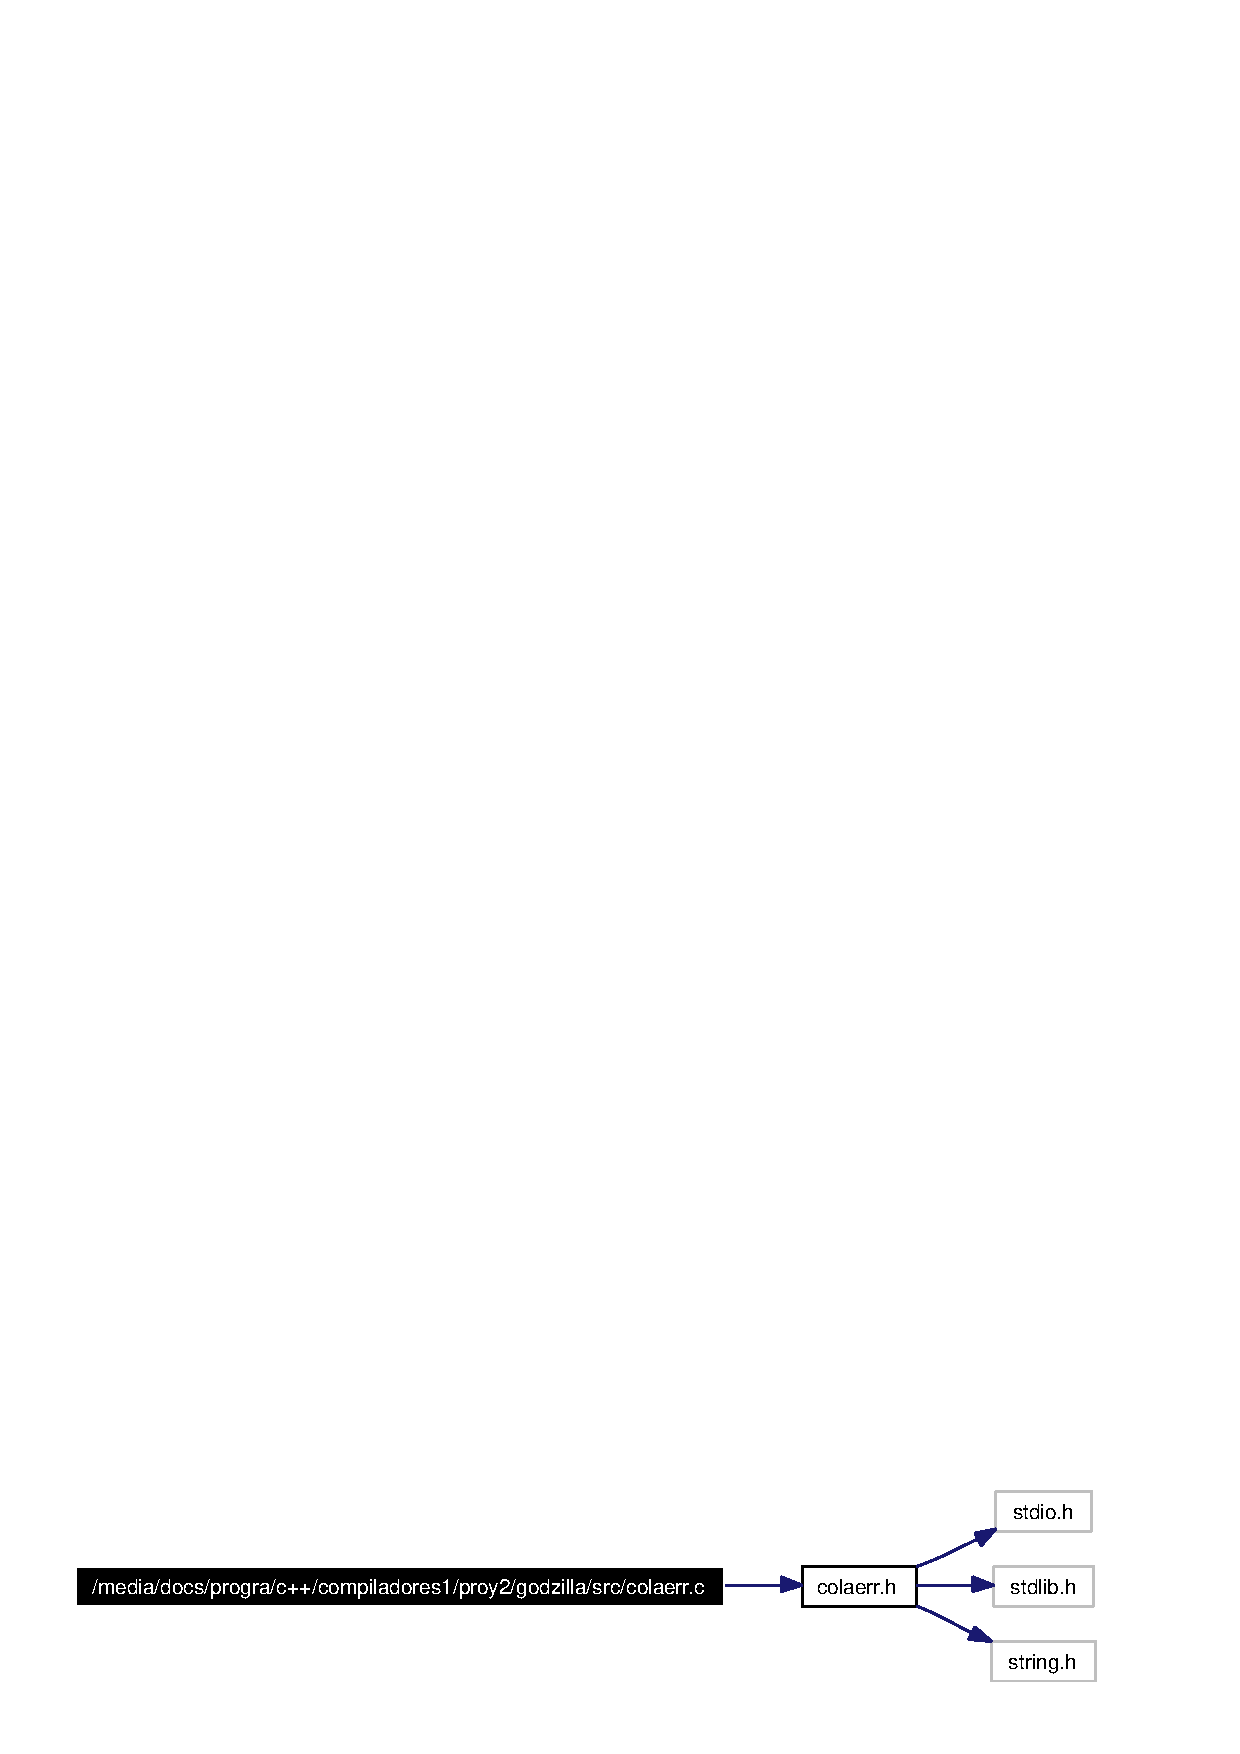
\includegraphics[width=263pt]{colaerr_8c__incl}
\end{center}
\end{figure}
\subsection*{Funciones}
\begin{CompactItemize}
\item 
void {\bf encolar\-Error} ({\bf cola\-Err} $\ast$cerr, {\bf tipo\-Error} $\ast$err)
\begin{CompactList}\small\item\em Agrega un error a la cola de errores. \item\end{CompactList}\item 
{\bf tipo\-Error} $\ast$ {\bf sacar\-Error} ({\bf cola\-Err} $\ast$cerr)
\begin{CompactList}\small\item\em Agrega un error a la cola de errores. \item\end{CompactList}\item 
void {\bf error\-Lexico} (char $\ast$msg)
\begin{CompactList}\small\item\em Devuelve primer error en la cola de erroes. \item\end{CompactList}\item 
void {\bf error\-Sintactico} (char $\ast$msg)
\begin{CompactList}\small\item\em Agrega mensaje a la cola de errores lexicos. \item\end{CompactList}\item 
void {\bf error\-Semantico} (char $\ast$msg, int num\-Linea)
\begin{CompactList}\small\item\em Agrega mensaje a la cola de errores sintacticos. \item\end{CompactList}\item 
int {\bf escribir\-Error\-Log\-XML} (const char $\ast$filename)
\begin{CompactList}\small\item\em Agrega mensaje a la cola de errores semanticos. \item\end{CompactList}\end{CompactItemize}
\subsection*{Variables}
\begin{CompactItemize}
\item 
static {\bf cola\-Err} {\bf errores\-Lexicos}
\item 
static {\bf cola\-Err} {\bf errores\-Sintacticos}
\item 
static {\bf cola\-Err} {\bf errores\-Semanticos}
\item 
static FILE $\ast$ {\bf errfile}
\item 
int {\bf hubo\-Error\-Sintactico} = 0
\item 
int {\bf hubo\-Error\-Semantico} = 0
\item 
int {\bf hubo\-Error\-Lexico} = 0
\end{CompactItemize}


\subsection{Descripci\'{o}n detallada}
Implementacion de la cola almacenadora de errores . 

Contiene rutinas de impresion hacia archivo XML 

Definici\'{o}n en el archivo {\bf colaerr.c}.

\subsection{Documentaci\'{o}n de las funciones}
\index{colaerr.c@{colaerr.c}!encolarError@{encolarError}}
\index{encolarError@{encolarError}!colaerr.c@{colaerr.c}}
\subsubsection{\setlength{\rightskip}{0pt plus 5cm}void encolar\-Error ({\bf cola\-Err} $\ast$ {\em cerr}, {\bf tipo\-Error} $\ast$ {\em err})}\label{colaerr_8c_a7}


Agrega un error a la cola de errores. 



Definici\'{o}n en la l\'{\i}nea 24 del archivo colaerr.c.

Hace referencia a nodo\-Cola\-Err::err, cola\-Err::primero, nodo\-Cola\-Err::siguiente, y cola\-Err::ultimo.

Referenciado por error\-Lexico(), error\-Semantico(), y error\-Sintactico().\index{colaerr.c@{colaerr.c}!errorLexico@{errorLexico}}
\index{errorLexico@{errorLexico}!colaerr.c@{colaerr.c}}
\subsubsection{\setlength{\rightskip}{0pt plus 5cm}void error\-Lexico (char $\ast$ {\em msg})}\label{colaerr_8c_a9}


Devuelve primer error en la cola de erroes. 



Definici\'{o}n en la l\'{\i}nea 53 del archivo colaerr.c.

Hace referencia a tipo\-Error::col, column, tipo\-Error::desc, encolar\-Error(), hubo\-Error\-Lexico, line\_\-num, y tipo\-Error::linea.\index{colaerr.c@{colaerr.c}!errorSemantico@{errorSemantico}}
\index{errorSemantico@{errorSemantico}!colaerr.c@{colaerr.c}}
\subsubsection{\setlength{\rightskip}{0pt plus 5cm}void error\-Semantico (char $\ast$ {\em msg}, int {\em num\-Linea})}\label{colaerr_8c_a11}


Agrega mensaje a la cola de errores sintacticos. 



Definici\'{o}n en la l\'{\i}nea 74 del archivo colaerr.c.

Hace referencia a tipo\-Error::col, tipo\-Error::desc, encolar\-Error(), hubo\-Error\-Semantico, y tipo\-Error::linea.

Referenciado por error().\index{colaerr.c@{colaerr.c}!errorSintactico@{errorSintactico}}
\index{errorSintactico@{errorSintactico}!colaerr.c@{colaerr.c}}
\subsubsection{\setlength{\rightskip}{0pt plus 5cm}void error\-Sintactico (char $\ast$ {\em msg})}\label{colaerr_8c_a10}


Agrega mensaje a la cola de errores lexicos. 



Definici\'{o}n en la l\'{\i}nea 63 del archivo colaerr.c.

Hace referencia a tipo\-Error::col, column, tipo\-Error::desc, encolar\-Error(), hubo\-Error\-Sintactico, line\_\-num, y tipo\-Error::linea.\index{colaerr.c@{colaerr.c}!escribirErrorLogXML@{escribirErrorLogXML}}
\index{escribirErrorLogXML@{escribirErrorLogXML}!colaerr.c@{colaerr.c}}
\subsubsection{\setlength{\rightskip}{0pt plus 5cm}int escribir\-Error\-Log\-XML (const char $\ast$ {\em filename})}\label{colaerr_8c_a12}


Agrega mensaje a la cola de errores semanticos. 



Definici\'{o}n en la l\'{\i}nea 84 del archivo colaerr.c.

Hace referencia a tipo\-Error::col, tipo\-Error::desc, errfile, tipo\-Error::linea, cola\-Err::primero, y sacar\-Error().\index{colaerr.c@{colaerr.c}!sacarError@{sacarError}}
\index{sacarError@{sacarError}!colaerr.c@{colaerr.c}}
\subsubsection{\setlength{\rightskip}{0pt plus 5cm}{\bf tipo\-Error}$\ast$ sacar\-Error ({\bf cola\-Err} $\ast$ {\em cerr})}\label{colaerr_8c_a8}


Agrega un error a la cola de errores. 



Definici\'{o}n en la l\'{\i}nea 36 del archivo colaerr.c.

Hace referencia a nodo\-Cola\-Err::err, cola\-Err::primero, nodo\-Cola\-Err::siguiente, y cola\-Err::ultimo.

Referenciado por escribir\-Error\-Log\-XML().

\subsection{Documentaci\'{o}n de las variables}
\index{colaerr.c@{colaerr.c}!errfile@{errfile}}
\index{errfile@{errfile}!colaerr.c@{colaerr.c}}
\subsubsection{\setlength{\rightskip}{0pt plus 5cm}FILE$\ast$ {\bf errfile}\hspace{0.3cm}{\tt  [static]}}\label{colaerr_8c_a3}




Definici\'{o}n en la l\'{\i}nea 17 del archivo colaerr.c.

Referenciado por escribir\-Error\-Log\-XML().\index{colaerr.c@{colaerr.c}!erroresLexicos@{erroresLexicos}}
\index{erroresLexicos@{erroresLexicos}!colaerr.c@{colaerr.c}}
\subsubsection{\setlength{\rightskip}{0pt plus 5cm}{\bf cola\-Err} {\bf errores\-Lexicos}\hspace{0.3cm}{\tt  [static]}}\label{colaerr_8c_a0}




Definici\'{o}n en la l\'{\i}nea 16 del archivo colaerr.c.\index{colaerr.c@{colaerr.c}!erroresSemanticos@{erroresSemanticos}}
\index{erroresSemanticos@{erroresSemanticos}!colaerr.c@{colaerr.c}}
\subsubsection{\setlength{\rightskip}{0pt plus 5cm}{\bf cola\-Err} {\bf errores\-Semanticos}\hspace{0.3cm}{\tt  [static]}}\label{colaerr_8c_a2}




Definici\'{o}n en la l\'{\i}nea 16 del archivo colaerr.c.\index{colaerr.c@{colaerr.c}!erroresSintacticos@{erroresSintacticos}}
\index{erroresSintacticos@{erroresSintacticos}!colaerr.c@{colaerr.c}}
\subsubsection{\setlength{\rightskip}{0pt plus 5cm}{\bf cola\-Err} {\bf errores\-Sintacticos}\hspace{0.3cm}{\tt  [static]}}\label{colaerr_8c_a1}




Definici\'{o}n en la l\'{\i}nea 16 del archivo colaerr.c.\index{colaerr.c@{colaerr.c}!huboErrorLexico@{huboErrorLexico}}
\index{huboErrorLexico@{huboErrorLexico}!colaerr.c@{colaerr.c}}
\subsubsection{\setlength{\rightskip}{0pt plus 5cm}int {\bf hubo\-Error\-Lexico} = 0}\label{colaerr_8c_a6}




Definici\'{o}n en la l\'{\i}nea 22 del archivo colaerr.c.

Referenciado por error\-Lexico().\index{colaerr.c@{colaerr.c}!huboErrorSemantico@{huboErrorSemantico}}
\index{huboErrorSemantico@{huboErrorSemantico}!colaerr.c@{colaerr.c}}
\subsubsection{\setlength{\rightskip}{0pt plus 5cm}int {\bf hubo\-Error\-Semantico} = 0}\label{colaerr_8c_a5}




Definici\'{o}n en la l\'{\i}nea 21 del archivo colaerr.c.

Referenciado por error\-Semantico().\index{colaerr.c@{colaerr.c}!huboErrorSintactico@{huboErrorSintactico}}
\index{huboErrorSintactico@{huboErrorSintactico}!colaerr.c@{colaerr.c}}
\subsubsection{\setlength{\rightskip}{0pt plus 5cm}int {\bf hubo\-Error\-Sintactico} = 0}\label{colaerr_8c_a4}




Definici\'{o}n en la l\'{\i}nea 20 del archivo colaerr.c.

Referenciado por error\-Sintactico().